\documentclass[11pt]{article}

\usepackage{comment} % enables the use of multi-line comments (\ifx \fi) 
\usepackage[a4paper,margin=1cm]{geometry}
\usepackage[utf8]{inputenc}
\usepackage[ngerman]{isodate}
\usepackage{gensymb}
\usepackage{graphicx}
\usepackage{booktabs}% http://ctan.org/pkg/booktabs
\usepackage{tabularx}
\usepackage{ltablex} % Longtables with tabularx
\usepackage[x11names]{xcolor}
\usepackage{amsmath}
\usepackage{amssymb}
\usepackage{amsthm}
\usepackage{array}
\usepackage{wrapfig}
\usepackage{subcaption}
\usepackage{csquotes}
\usepackage{lscape}
\usepackage{geometry}
\usepackage{multicol}
\usepackage{bm}
\usepackage{enumitem}
\usepackage{hyperref}
\usepackage{mdframed}
\usepackage{scalerel}
\usepackage{stackengine}
\usepackage{mathtools}
\usepackage{pdfpages}

% Code highlighting
\usepackage{minted}
\surroundwithmdframed{minted}

% Be able to caption equations and float them in place
\usepackage{float}

\newmdtheoremenv{theorem}{Theorem}

\theoremstyle{definition}
\newmdtheoremenv{definition}{Definition}[section]


\geometry{a4paper, margin=2.4cm}

\newcommand\equalhat{\mathrel{\stackon[1.5pt]{=}{\stretchto{\scalerel*[\widthof{=}]{\wedge}{\rule{1ex}{3ex}}}{0.5ex}}}}
\newcommand\defeq{\mathrel{\overset{\makebox[0pt]{\mbox{\normalfont\tiny def}}}{=}}}
\newcolumntype{C}{>{\centering\arraybackslash}X}

\newcommand*\samplemean[1]{\overline{#1}}
\newcommand*\ev[1]{\mathrel{\text{E}\left[#1\right]}}
\newcommand*\R{\mathbb{R}}
\newcommand*\Z{\mathbb{Z}}
\newcommand*\N[1]{\mathcal{N}\left(#1\right)}
\newcommand*\Likelihood{\mathcal{L}}
\newcommand*\diff{\mathop{}\!\mathrm{d}}
\newcommand*\Diff[1]{\mathop{}\!\mathrm{d^#1}}
\newcommand*\Exp[1]{\mathop{\text{Exp}}\left(#1\right)}
\newcommand*\Cov[1]{\mathop{\text{Cov}}\left(#1\right)}
\newcommand*\Cor[1]{\mathop{\text{Cor}}\left(#1\right)}
\newcommand*\Var[1]{\mathop{\text{Var}}\left(#1\right)}

\DeclarePairedDelimiter\abs{\lvert}{\rvert}
\DeclarePairedDelimiter\norm{\lVert}{\rVert}

\setcounter{tocdepth}{3}
\setcounter{secnumdepth}{3}

\graphicspath{{./img/}}

\begin{document}
	
\title{Applied Statistics and Data Analysis HS20}
\author{Pascal Baumann\\pascal.baumann@stud.hslu.ch}
\maketitle



For errors or improvement raise an issue or make a pull request on the \href{https://github.com/KilnOfTheSecondFlame/mse_summaries}{github repository}.

\tableofcontents
\newpage

\section{Introduction}
This is module concerns itself with quality control, especially with \textbf{statistical quality control}. Statistical process control is understood to be

\begin{definition}
	Statistical process control is, first and foremost, a way of thinking which happens to have some tools attached.
\end{definition}

\section{Statistical Process and Quality Control}
These tools are seven statistical methods for analysing data colloquially known as \textbf{magnificent seven}:
\begin{enumerate}[noitemsep]
	\item histogram
	\item check sheet
	\item Pareto chart
	\item defect concentration diagram
	\item cause-and-effect diagram
	\item control chart
	\item scatter diagram
\end{enumerate}

\subsubsection{Check Sheet}
The check sheet is a simple method of quality control and consists of a form for  registering and counting possible problems in a production process.

\subsubsection{Pareto Chart}
The Pareto chart is the application of the Pareto principle which states that \emph{80 percent of the result can be achieved with 20 percent of the commitment}. The numbers are arbitrarily chosen, but show up in this magnitude in many real world applications.

\subsection{Location Plot}
The location plot is also called the defect concentration diagram, and is used to graphically visualise the locations of various defects on the physical object.

\begin{figure}[H]
	\centering
	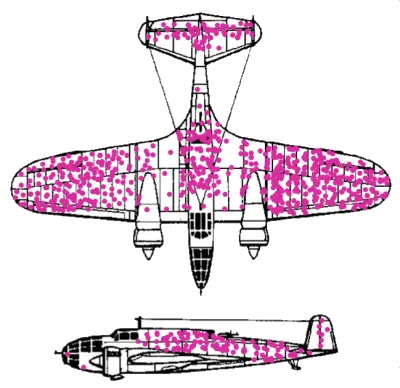
\includegraphics[width=0.5\linewidth]{img/bullet_holes_wwii}
	\caption{Bullet holes found in WWII allied bombers which returned after sorties}
	\label{fig:bulletholeswwii}
\end{figure}

\subsubsection{Cause-and-Effect Diagram}
This tool has the form of a fishbone diagram and is used for the systematic identification of causes resulting in problems.

\subsection{Construction of Control Charts}
The basis for control charts is the idea that a process can run according to specifications or outside of them. These are upper and lower bound and are derived statistically. The process is then continuously monitored and plotted against these bounds. The range between the limits is called \textbf{control area}.

\begin{figure}[tbh]
	\centering
	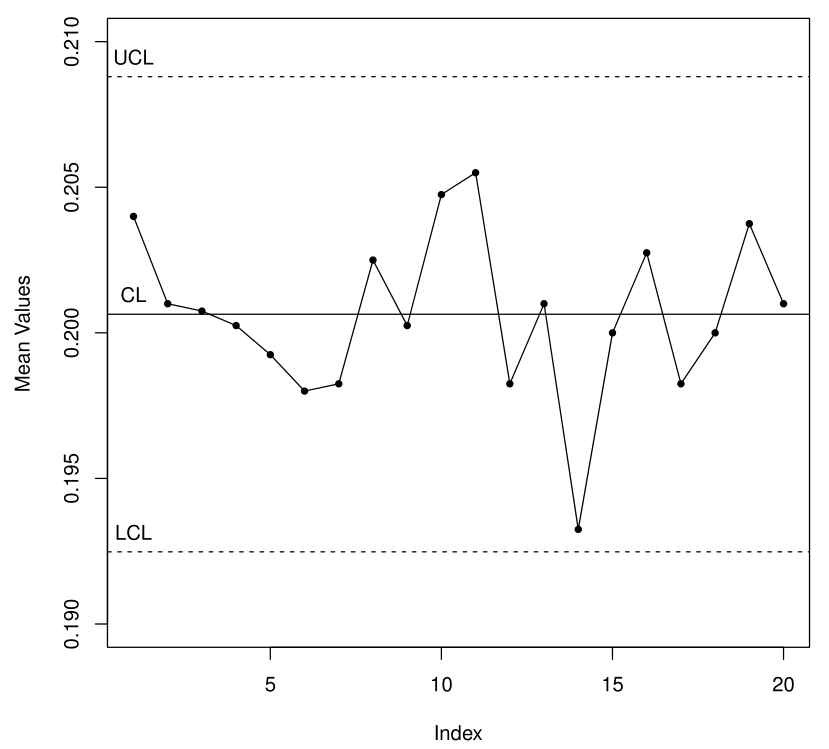
\includegraphics[width=0.5\linewidth]{img/control_chart}
	\caption{Sample control chart with UCL and LCL indicated}
	\label{fig:controlchart}
\end{figure}

The distance between upper control limit (UCL) and lower control limit (LCL) is three times the standard deviation.
\begin{align*}
	\text{LCL} &= \mu_0 - z_q \frac{\sigma}{\sqrt{n}}\\
	\text{UCL} &= \mu_0 + z_q \frac{\sigma}{\sqrt{n}}
\end{align*}

\subsubsection{Shewhart Control Charts}
The problem with constructing the control chart is that mean and standard deviation of a process are generally unknown. Shewhart solves this by first monitoring the variation and then the mean of a process. Sample the process periodically under the assumption that the process is normally distributed.
\begin{enumerate}
	\item Calculate the mean of each sample
	\begin{equation*}
		\samplemean{x}_i = \frac{1}{n}\sum_{j=1}^{n}x_{ij}
	\end{equation*}
	\item Calculate standard deviation of the samples
	\begin{equation*}
		s_i = \sqrt{\frac{1}{n-1} \sum_{j=1}^{n}(x_{ij}-\samplemean{x}_i)^2}
	\end{equation*}
	\item Calculate the range R for each sample
	\begin{equation*}
		R_i = \max(x_{ij}) - \min(x_{ij}) \qquad j\in1..n
	\end{equation*}
\end{enumerate}

\paragraph{Construction of an $R$ chart} Take the data from the trial run with $k$ samples of sample size $n$ from the process under supervision. The centreline (CL) of the process is denoted by $\samplemean{R}$ and calculated as follows
\begin{equation*}
	\samplemean{R} = \frac{1}{k}\sum_{i=1}^{k}R_i
\end{equation*}
The standard deviation of the statistic $\samplemean{R}$ is denoted $\sigma_R$. The control limits of the $R$ chart can then be calculated
\begin{align}
	\text{LCL} &= D_3\samplemean{R}\\
	\text{UCL} &= D_4\samplemean{R}\\
\end{align}
The constants $D_3$ and $D_4$ are dependent on the sample size $n$ and must be looked up in a specific table.

After the centreline and the control limits are determined the ranges $R_i$ are sequentially entered against the index $i$ in a scatter plot. In addition, lines for the control limits UCL and LCL are drawn into the same graph. If a sample is outside the control area, the sample is omitted and the limits recalculated.

\paragraph{Construction of an $\samplemean{x}$ chart} The control limits of an $\samplemean{x}$ chart are based on the three sigma limits of the empirical distribution of the statistic $\samplemean{x}$.

The control limits are then
\begin{align}
	\text{LCL} &= \mu - 3 \frac{\sigma}{\sqrt{n}}\\
	\text{UCL} &= \mu + 3 \frac{\sigma}{\sqrt{n}}
\end{align}
The assumption is that the $R$ chart is under statistical control and the real value of $\sigma$ can thus be approximated by
\begin{equation*}
	\hat{\sigma} = \frac{\samplemean{R}}{d_2}
\end{equation*}
as it is a reliable estimate for the process deviation. The constant $d_2$ is again dependent on the sample size $n$ and can be found in the table.

Any samples excluded for the construction of the $R$ chart, should also be disregarded for the construction of the $\samplemean{x}$ chart. This results in a data set of $k^\star$ valid samples and a corrected estimate for $\mu$
\begin{equation*}
	\samplemean{\samplemean{x}} = \frac{1}{k^\star}\sum_{i=1}^{k^\star}\samplemean{x}_i
\end{equation*}
and the corrected control limits
\begin{align*}
	\text{LCL} &= \samplemean{\samplemean{x}} - 3 \frac{\samplemean{R}}{d_2}\frac{1}{\sqrt{n}} \approx \samplemean{\samplemean{x}} - A_2\samplemean{R} \\
	\text{UCL} &= \samplemean{\samplemean{x}} + 3 \frac{\samplemean{R}}{d_2}\frac{1}{\sqrt{n}} \approx \samplemean{\samplemean{x}} + A_2\samplemean{R}
\end{align*}

\paragraph{Construction of $\samplemean{x}$ and $s$} As there are different ways to measure the variation of a process, a number of different control charts may be employed. One combination that is often used is the $\samplemean{x}$ and $s$ charts. The construction of these two is similar to $\samplemean{x}$ based on $R$, again, the variation is brought under control and then the process standard deviation is estimated using the $\samplemean{x}$ chart.

The centreline of the $s$ chart is denoted $\samplemean{s}$ and is calculated from the standard deviations $s_i$ of the $k$ samples as follows
\begin{equation*}
	\samplemean{s} = \frac{1}{k}\sum_{i=1}^{k} s_i
\end{equation*}
The control limits are then
\begin{align*}
	\text{LCL} &= B_3\samplemean{s}\\
	\text{UCL} &= B_4\samplemean{s}\\
\end{align*}
After the centre line and control limits are determined, the sample standard deviation and lines are plotted in a scatter diagram. Any observation falling outside the control area are omitted and the ranges recalculated.

\paragraph{Construction of $\samplemean{x}$ based on $s$} Using an $s$ chart that is \textbf{under control} the process standard deviation can be estimated by
\begin{equation*}
	\hat{\sigma} = \frac{\samplemean{s}}{c_4}
\end{equation*}
As before, Any samples that were excluded for construction of the $s$ chart should also be disregarded for the construction of the $\samplemean{x}$ chart.

The mean values of the resulting $k^\star$ samples give an estimation of $\mu$
\begin{equation*}
	\samplemean{\samplemean{x}} = \frac{1}{k^\star}\sum_{i=1}^{k^\star}\samplemean{x}_i
\end{equation*}
The control limits are then
\begin{align*}
	\text{LCL} &= \samplemean{\samplemean{x}} - 3 \frac{\samplemean{s}}{c_4}\frac{1}{\sqrt{n}} \approx \samplemean{\samplemean{x}} - A_3\samplemean{s}\\
	\text{UCL} &= \samplemean{\samplemean{x}} + 3 \frac{\samplemean{s}}{c_4}\frac{1}{\sqrt{n}} \approx \samplemean{\samplemean{x}} + A_3\samplemean{s}
\end{align*}

\subsubsection{Individuals Control Charts}
Often its not practical to pick several production pieces for a sample data set, for example if a process is very slow (for example Falcon Heavy Boosters) or if the difference of a repeated measurement cannot be attributed to the process variation, but to the measuring methods. In such situations, it is reasonable to construct a control chart for individual measurements.

The problem that arises is that the variability of the process cannot be estimated from a single measurement. The solution is to use a moving range
\begin{equation*}
	MR_i = \abs{x_{i+1} + x_i}\quad \forall i\in1..n-1
\end{equation*}
The process standard deviation can be estimated from the arithmetic mean of the moving ranges
\begin{equation*}
	\samplemean{MR} = \frac{1}{n-1}\sum_{i=1}^{n-1}MR_i
\end{equation*}
\begin{equation*}
	\hat{\sigma} = \frac{\samplemean{MR}}{d_2}
\end{equation*}
With $d_2$ dependent on the sample size $n$, which would be two in this case as two neighbouring samples were used to calculate the moving range.
The centreline $samplemean{x}$ is the arithmetic mean of the measured values
\begin{equation*}
	\samplemean{x} = \frac{1}{n}\sum_{i=1}^{n}x_i
\end{equation*}
And the control limits
\begin{align*}
	\text{LCL} &= \samplemean{x} - 3\frac{\samplemean{MR}}{d_2}\\
	\text{UCL} &= \samplemean{x} + 3\frac{\samplemean{MR}}{d_2}
\end{align*}

\subsubsection{$p$ Control Chart}
Often we are only interested if a product is usable or defective, which makes the proportion of defectives to tested a discrete random variable. Thus a control chart for attributes data, the $p$ chart, can be used. This chart is cheaper and easier to use, but needs a bigger sample size $n$ than the Shewhart charts.

\vspace{1em}
\noindent
An estimator of success probability is the relative frequency
\begin{equation*}
	\hat{p} = \frac{D}{n}
\end{equation*}
And the variance then
\begin{equation*}
	\Var{\hat{p}} = \frac{p(1-p)}{n}
\end{equation*}
The centre line and the control limits are again determined from a \textbf{stable trial run} with $k^\star$ valid samples. In the event that all $n_i$ are equal
\begin{align*}
	\samplemean{p} &= \frac{1}{k^\star}\sum_{i=1}^{k^\star}p_i\\
	\text{LCL} &= \samplemean{p} - 3 \sqrt{\frac{\samplemean{p}(1-\samplemean{p})}{n}}\\
	\text{UCL} &= \samplemean{p} + 3 \sqrt{\frac{\samplemean{p}(1-\samplemean{p})}{n}}
\end{align*}
In the event that not all $n_i$ are equal
\begin{align*}
	\samplemean{p} &= \frac{d_1 + d_2 + \dots + d_{k^\star}}{n_1 + n_2 + \dots + n_{k^\star}}\\
	\text{LCL}_i &= \samplemean{p} - 3 \sqrt{\frac{\samplemean{p}(1-\samplemean{p})}{n}}\\
	\text{UCL}_i &= \samplemean{p} + 3 \sqrt{\frac{\samplemean{p}(1-\samplemean{p})}{n}}
\end{align*}
The control limits now depend on the index $i$. It might happen that for small sample sizes $n_i$ the control limits $\text{LCL}_i$ are negative, which obviously makes no sense in the context of a probability, in thus correct $\text{LCL}_i$ to $0$.

\section{Multiple Regression}

\section{Design of Experiments}

\end{document}
